\renewcommand\figuresI{

  \renewcommand\w{0.3\linewidth}
  \renewcommand\fw{0.9\textwidth}

  \begin{figure}[H]
    \centering
    \begin{minipage}[b]{\w}
      \centering
      \label{surface:1}
      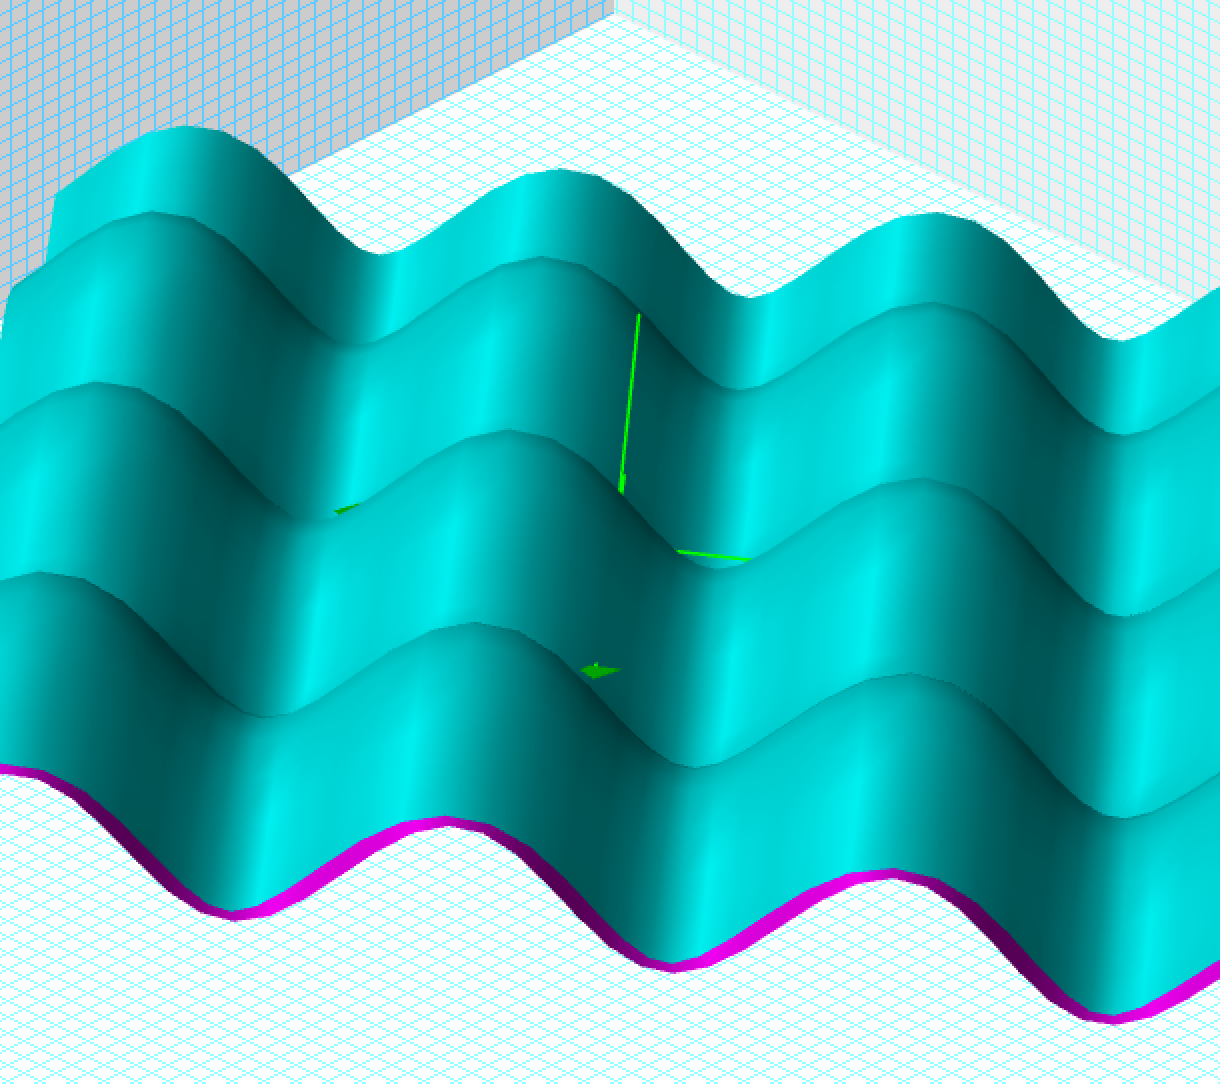
\includegraphics[width=\fw]{img/16-surface/01.png}
      \caption{Caption}
      \vspace{4ex}
    \end{minipage} % end
    \begin{minipage}[b]{\w}
      \centering
      \label{surface:2}
      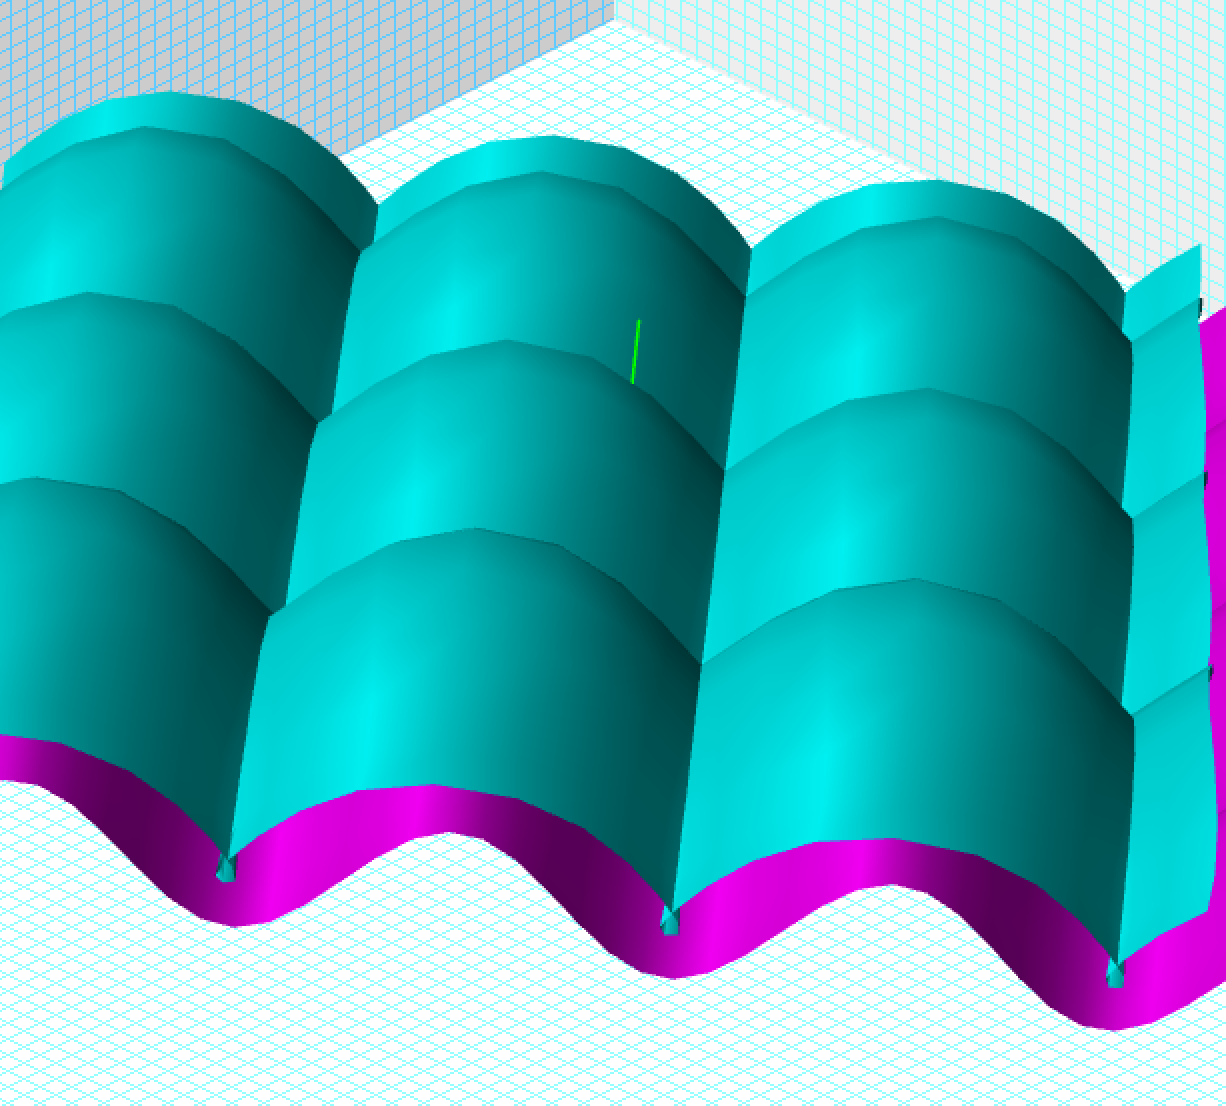
\includegraphics[width=\fw]{img/16-surface/02.png}
      \caption{Caption}
      \vspace{4ex}
    \end{minipage} % end
    \begin{minipage}[b]{\w}
      \centering
      \label{surface:3}
      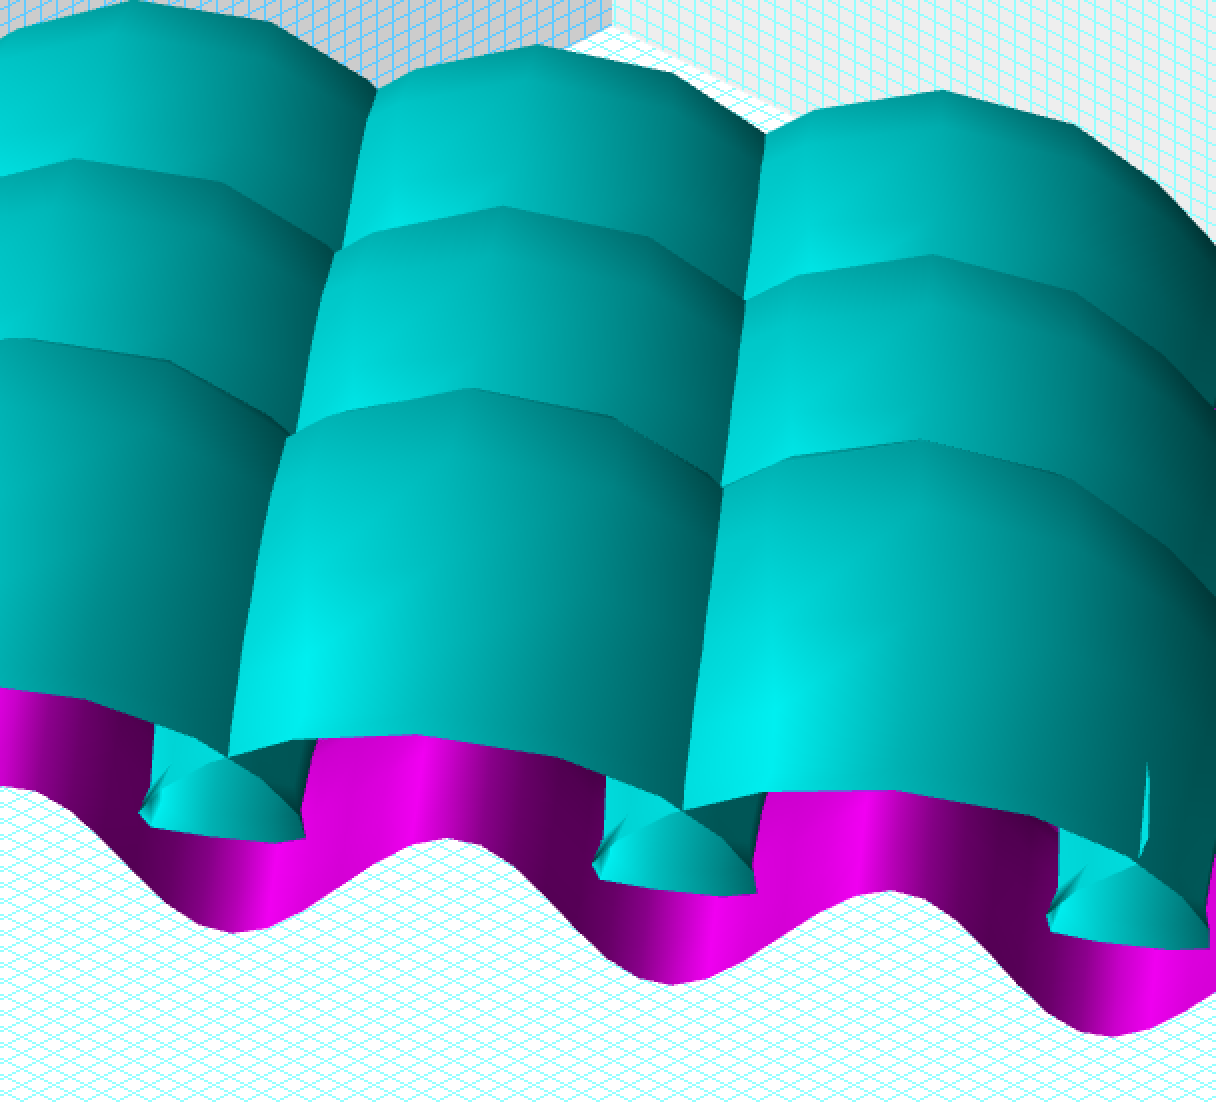
\includegraphics[width=\fw]{img/16-surface/03.png}
      \caption{Caption}
      \vspace{4ex}
    \end{minipage} % end
    \begin{minipage}[b]{\w}
      \centering
      \label{surface:4}
      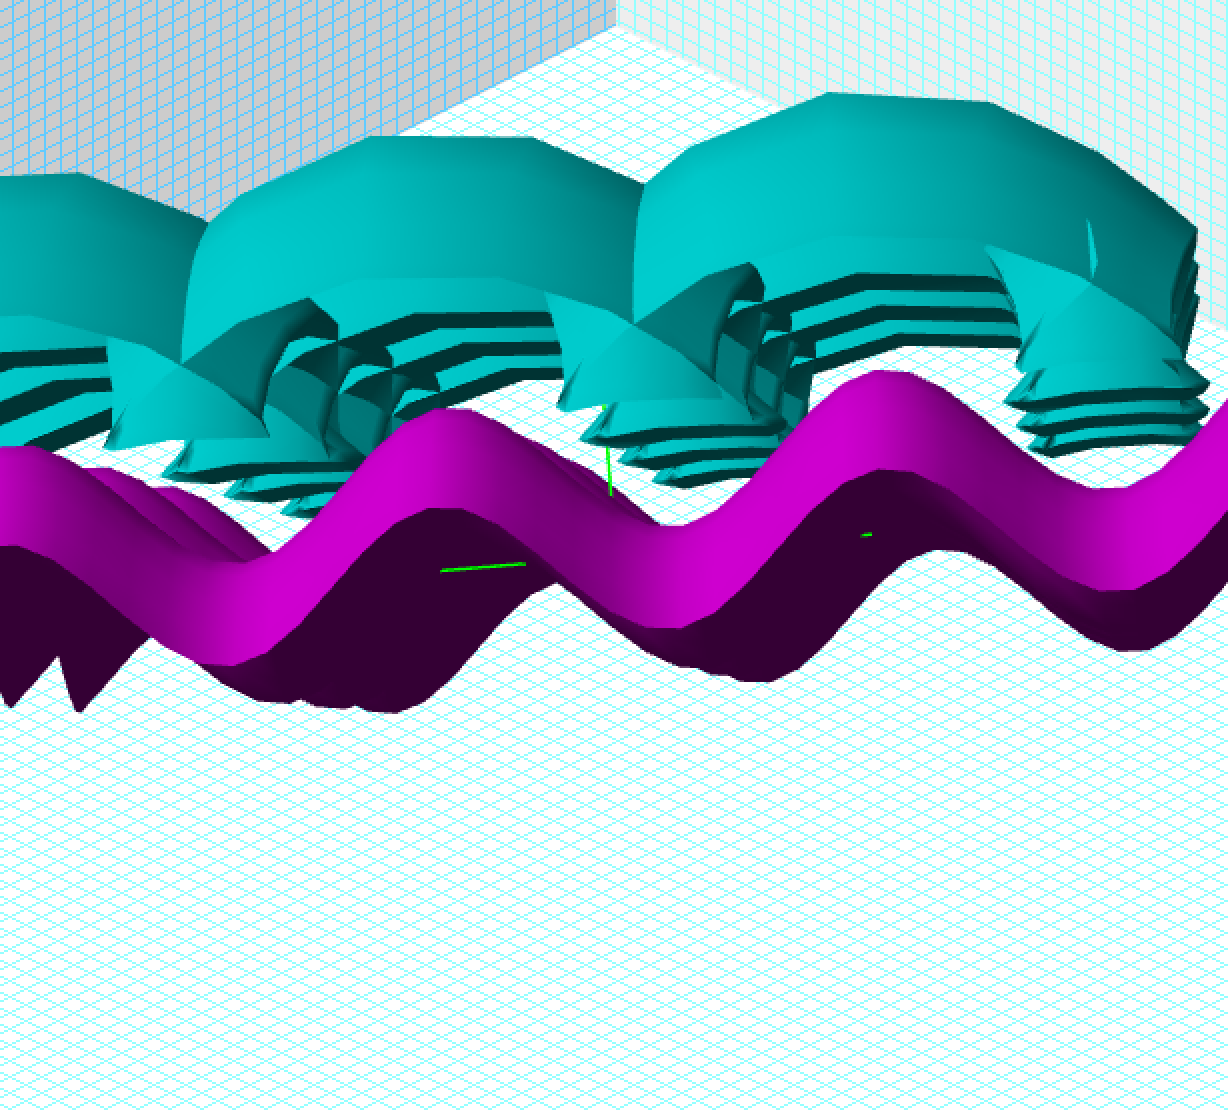
\includegraphics[width=\fw]{img/16-surface/04.png}
      \caption{Caption}
      \vspace{4ex}
    \end{minipage} % end
    \begin{minipage}[b]{\w}
      \centering
      \label{surface:5}
      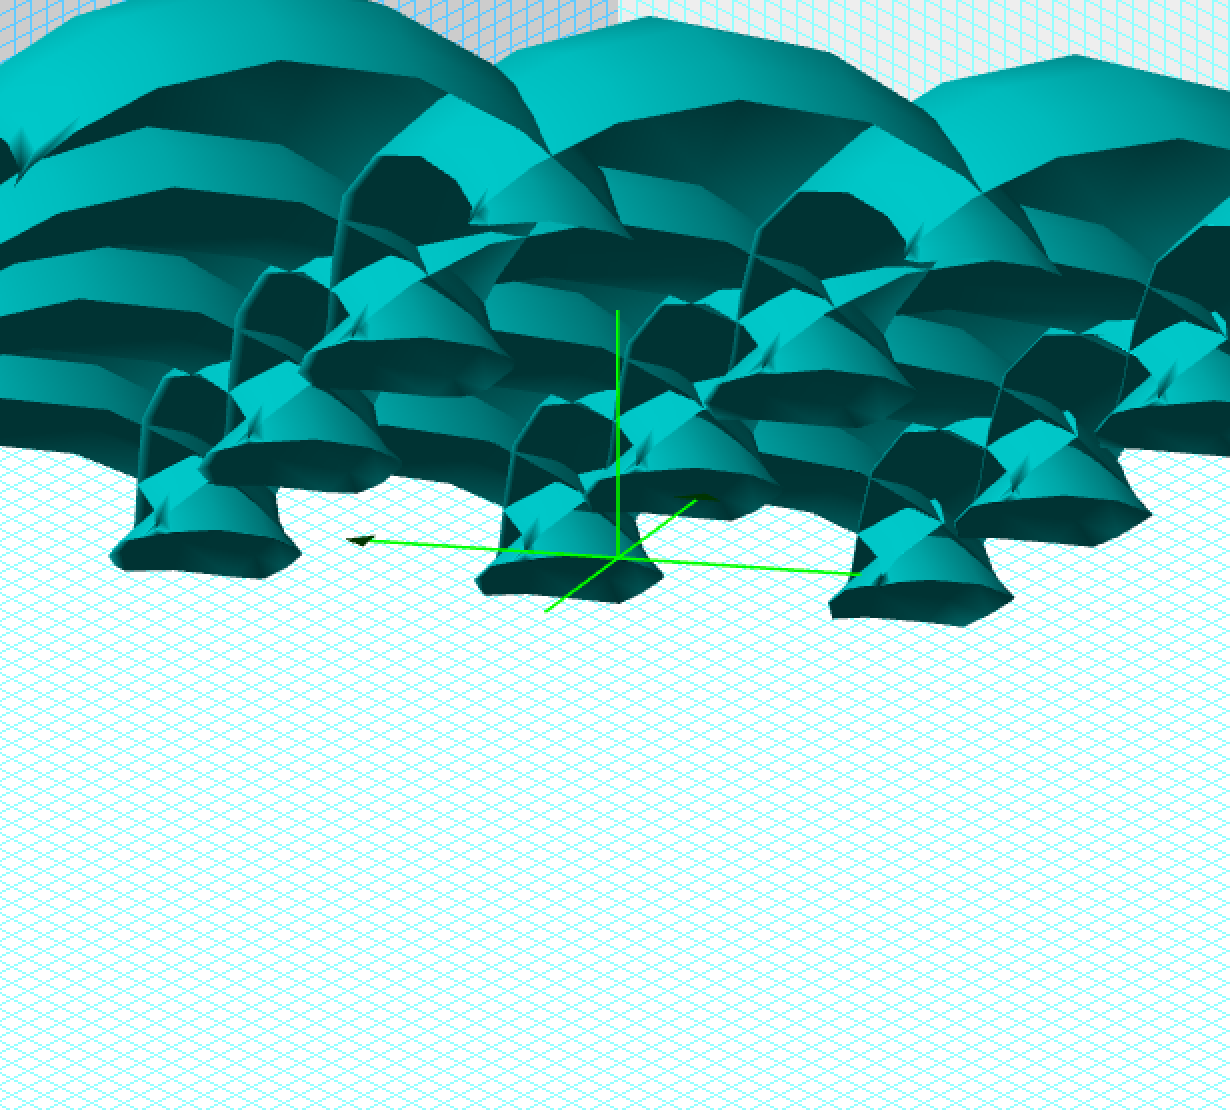
\includegraphics[width=\fw]{img/16-surface/05.png}
      \caption{Caption}
      \vspace{4ex}
    \end{minipage} % end
  \end{figure}

}

\renewcommand\figuresII{

  \renewcommand\w{0.4\linewidth}
  \renewcommand\fw{0.9\textwidth}

  \begin{figure}[H]
    \centering
    \begin{minipage}[b]{\w}
      \centering
      \label{surface:6}
      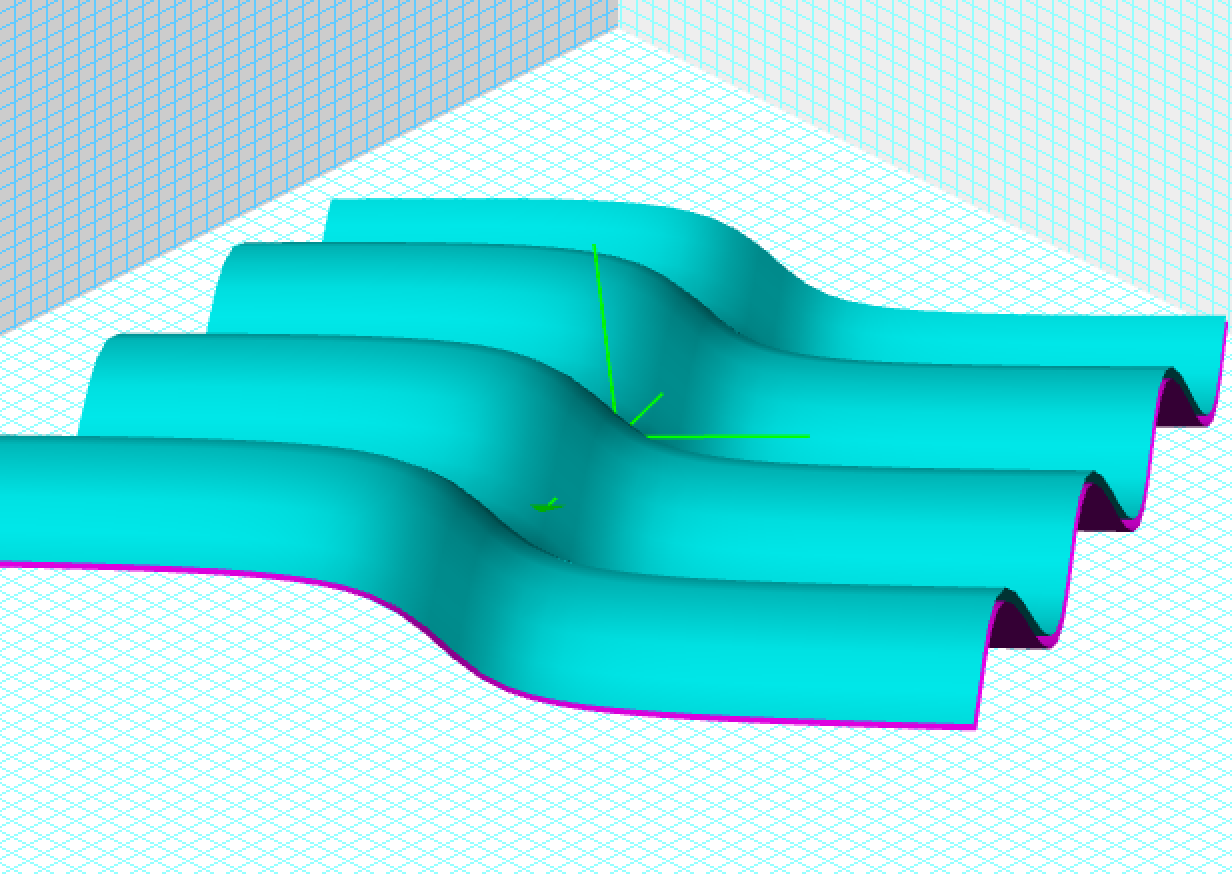
\includegraphics[width=\fw]{img/16-surface/06.png}
      \caption{Caption}
      \vspace{4ex}
    \end{minipage} % end
    \begin{minipage}[b]{\w}
      \centering
      \label{surface:7}
      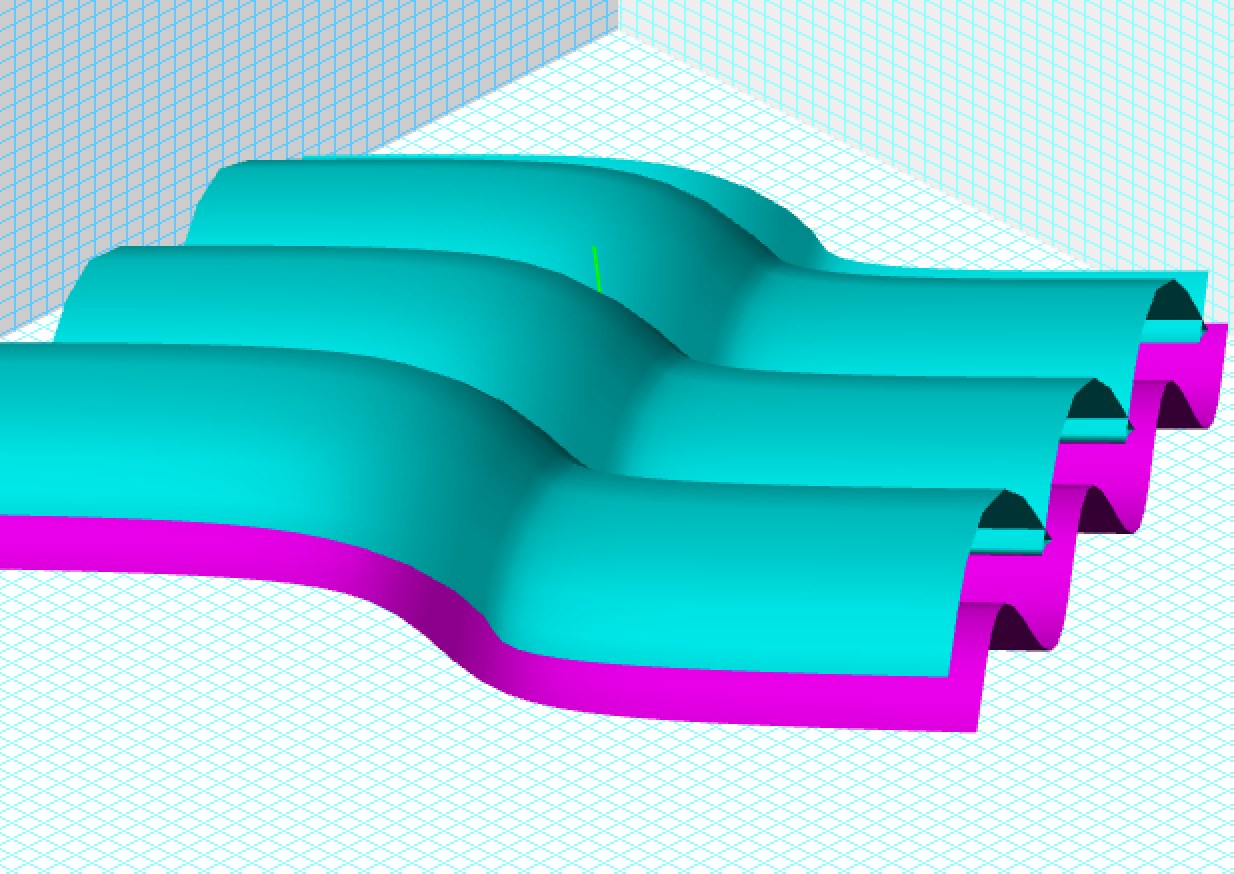
\includegraphics[width=\fw]{img/16-surface/07.png}
      \caption{Caption}
      \vspace{4ex}
    \end{minipage} % end
    \begin{minipage}[b]{\w}
      \centering
      \label{surface:8}
      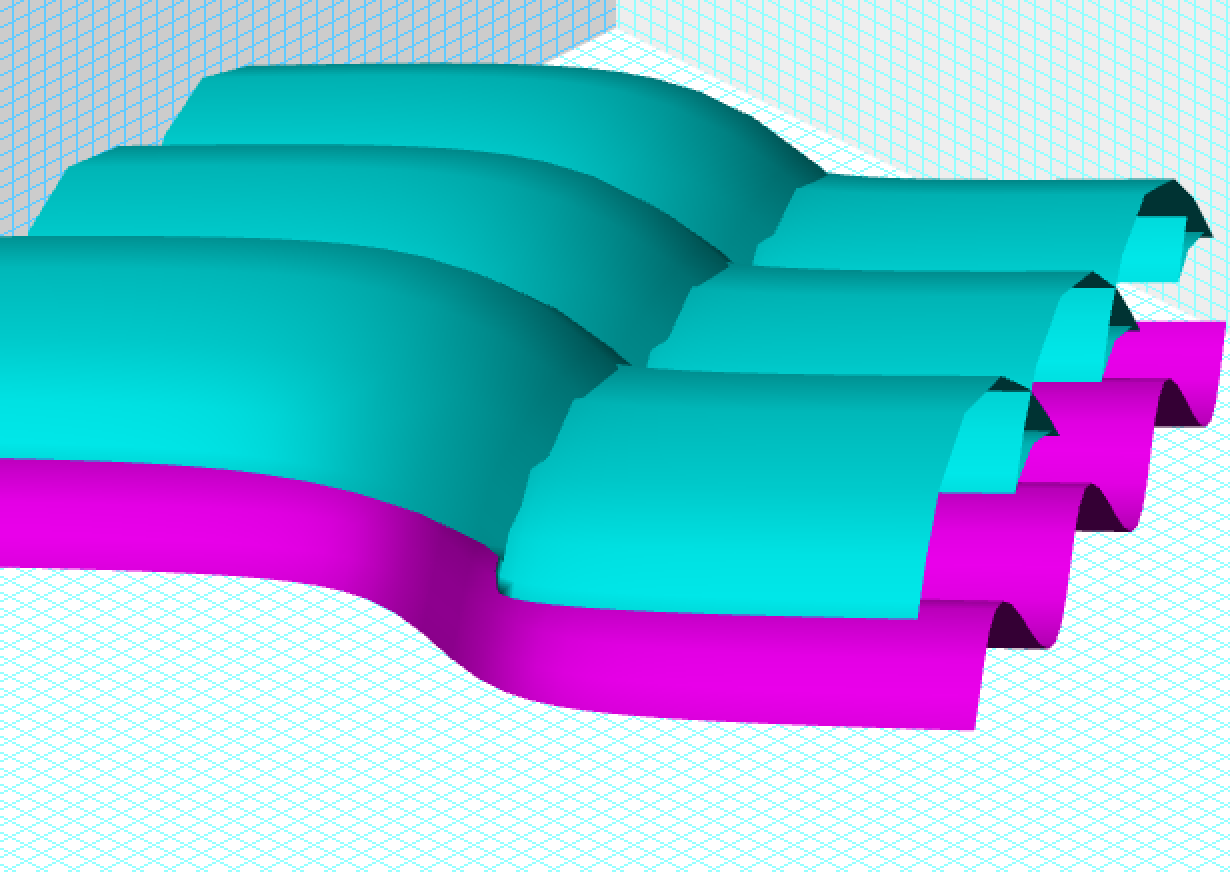
\includegraphics[width=\fw]{img/16-surface/08.png}
      \caption{Caption}
      \vspace{4ex}
    \end{minipage} % end
    \begin{minipage}[b]{\w}
      \centering
      \label{surface:9}
      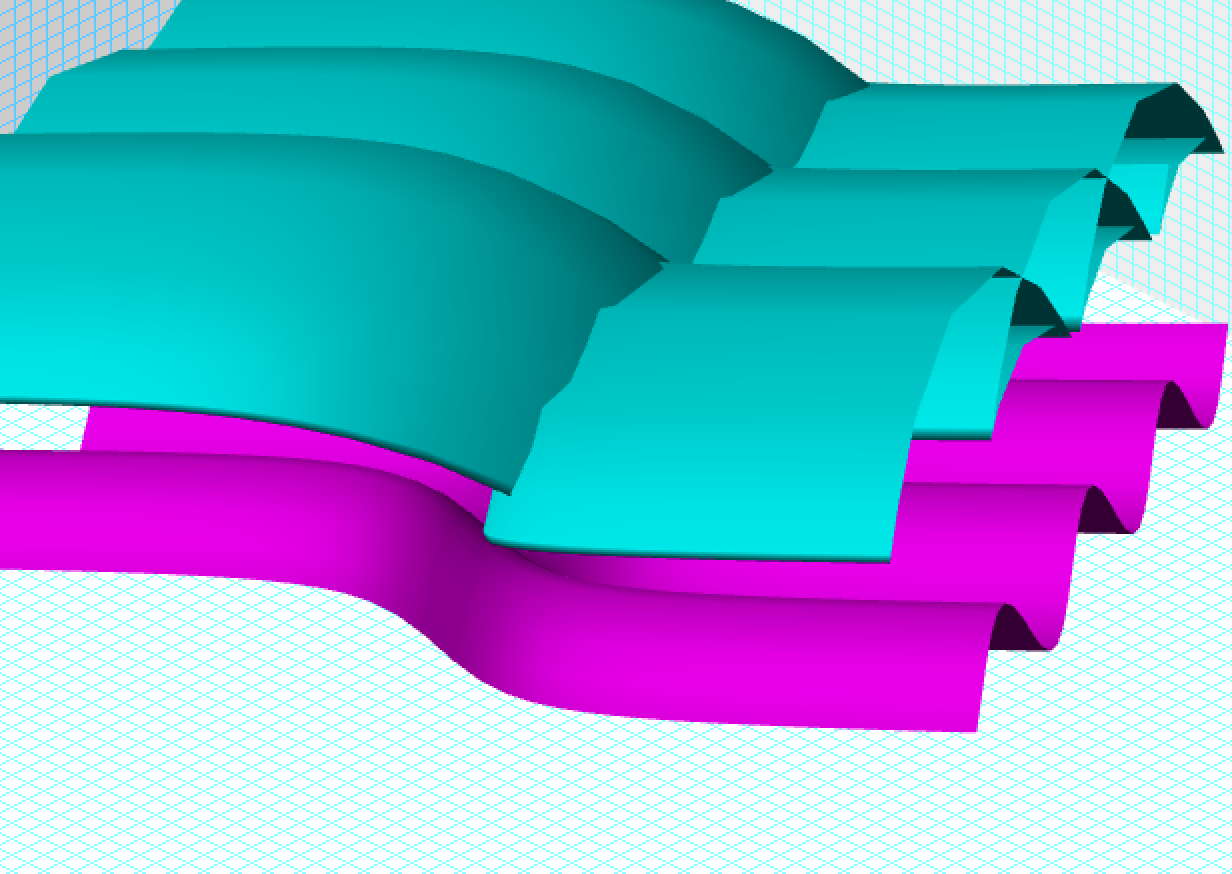
\includegraphics[width=\fw]{img/16-surface/09.png}
      \caption{Caption}
      \vspace{4ex}
    \end{minipage} % end
  \end{figure}

}

\section{The 3-Dimensional Case - N-Units Away Surfaces}

One last thing I want to mention is that you can, with only minimal effort, extend almost all of the ideas covered in this paper to higher dimensional arenas. Where before we were taking a function $y = f(x)$ and moving one unit away along every normal line to that function, now take a surface $z = f(x, y)$ and move one unit away from it along every normal line.

\renewcommand\bvec{\langle -f'(t), 1 \rangle}
\newcommand\IIIdvec{\langle -\dfrac{df}{dx}, -\dfrac{df}{dy}, 1 \rangle}

Instead of $f_N(t) =
\begin{bmatrix}
  t \\
  f(t)
\end{bmatrix} + \dfrac{ N }{ |\bvec| } \bvec $, now we have $ f_N(u, v) =
\begin{bmatrix}
  u \\
  v \\
  f(u, v)
\end{bmatrix} + \allowbreak \dfrac{ N }{ |\IIIdvec| } \allowbreak \IIIdvec $.

Running this into the Pacific Tech Graphing Calculator, one gets a glimpse at the marvelous and humorous world of $N$-Units Away Surfaces! Here is the graph of the $N$-Units Away Surfaces for $f(x, y) = sinx + siny$:

\figuresI

While these are the N-Units Away Surfaces for $f(x, y) = atan(x) + sin(y)$:

\figuresII
